\noindent
\subsection{Identifying anomalous Editors and Reviewers}
\label{prediction}

%[{\color{red}{\bf Shall ckeck the rest from here after you have a complete version.}}]

In the previous sections we discussed how different factors indicate anomalous behavior of referees and editors. In this section, we check whether we can use them to automatically differentiate between normal and anomalous editors and referees. We propose separate unsupervised models for editors and reviewers.

\begin{figure}
\centering
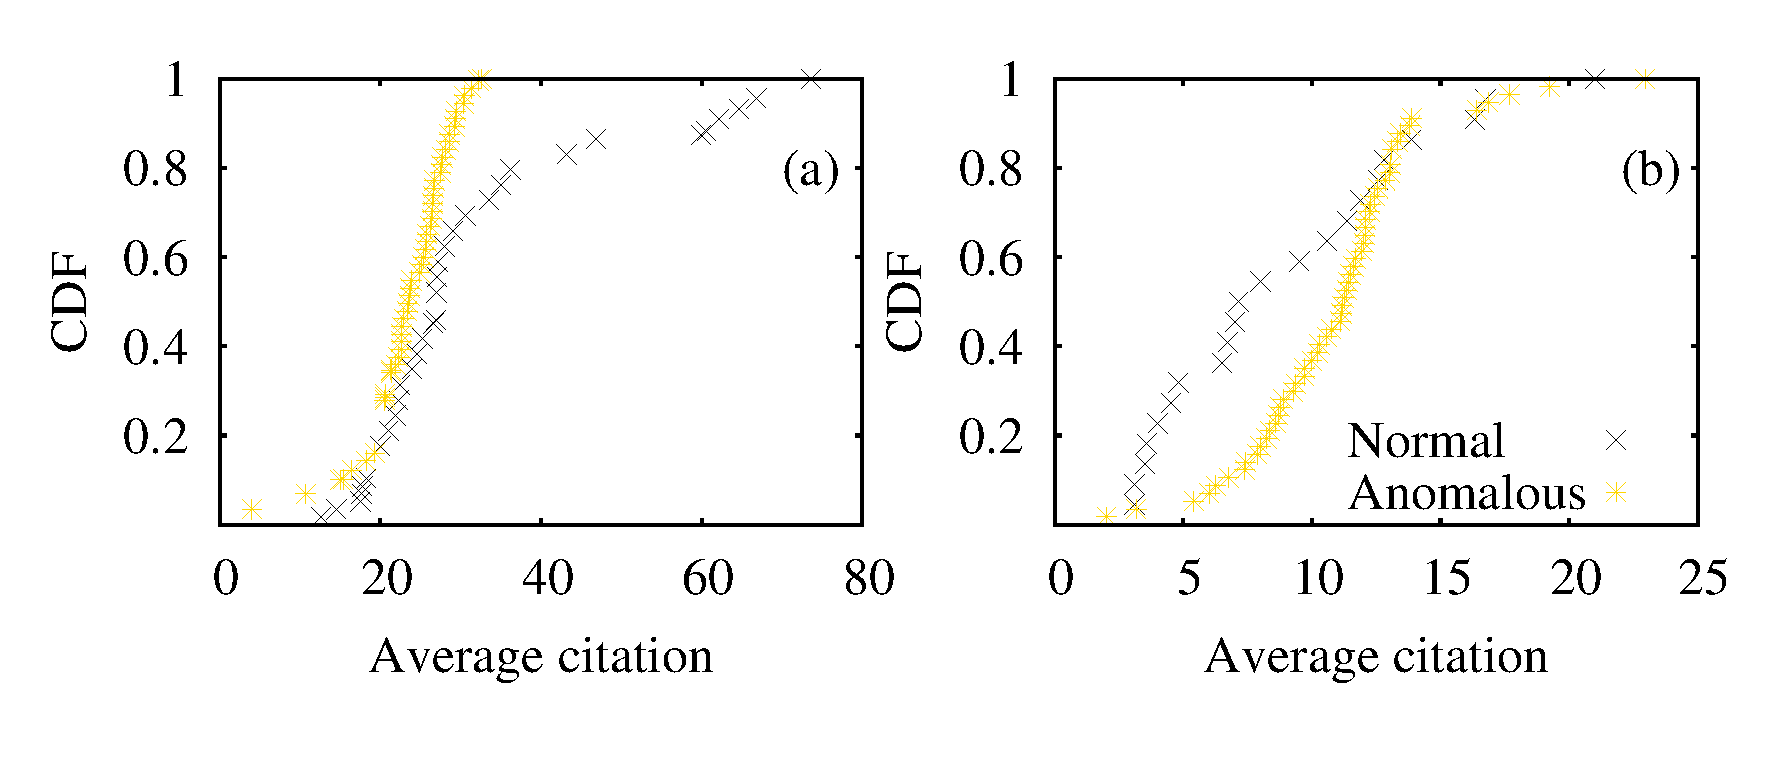
\includegraphics[scale=0.27]{./texfiles/Chapter_4/cikm/figures/editor_all_anom.eps}
\caption{\label{ed_pred}Cumulative distribution function of the average citations for the two sets of editors (anomalous and normal).\vspace{4mm}} 
\end{figure}


\subsubsection{Editors}
For each editor $i$, we measure $MEAT_{i}$, $RDI_{i}$, $RADI_{i}$ and $SRI_{i}$ which form a feature vector. 
%[{\color{red}{\bf Have you not used $SRI$? Why?}}] 
We also consider the editors who were assigned at least 5 papers and accepted at least 1 paper before 2013. 
To detect anomalies we use the 
$k-means$ clustering setting with $k=2$. The two clusters are of sizes 25 and 68 respectively. Clearly this set of 25 editors are the anomalous ones.
In figure \ref{ed_pred} we plot the cumulative distribution of average citation of accepted (figure \ref{ed_pred}(a)) and rejected  (figure \ref{ed_pred}(b)) papers. We observe that citation of accepted papers assigned to anomalous editors are significantly lower while citation of rejected papers are significantly higher compared to those assigned to normal editors.


\subsubsection{Reviewers}

Similarly for each reviewer $i$ we associate a feature vector of size seven consisting of $MRAT_{i}$, $MRSD_{i}$, $TDI_{i}$, $EDI_{i}$, $AR_{i}$, $MTD_{i}$ and $DFI_{i}$. 
%[{\color{red}{\bf Have you not used $DFI$? Why?}}] 
We filter out reviewers who have reviewed at least 5 papers and accepted at least 1 before 2013. This reduces our set of reviewers to 2328. By using $k-means$ clustering ($k=2$), we obtain two clusters of size 339 and 
1999. On plotting cumulative distribution of the average citation for accepted (refer to figure \ref{rev_pred}(a)) and rejected papers (refer to figure \ref{rev_pred}(b)), we observe that the papers accepted by anomalous reviewers are cited significantly lesser while those rejected by them are cited significantly higher compared to the normal referees.

\begin{figure}
\centering
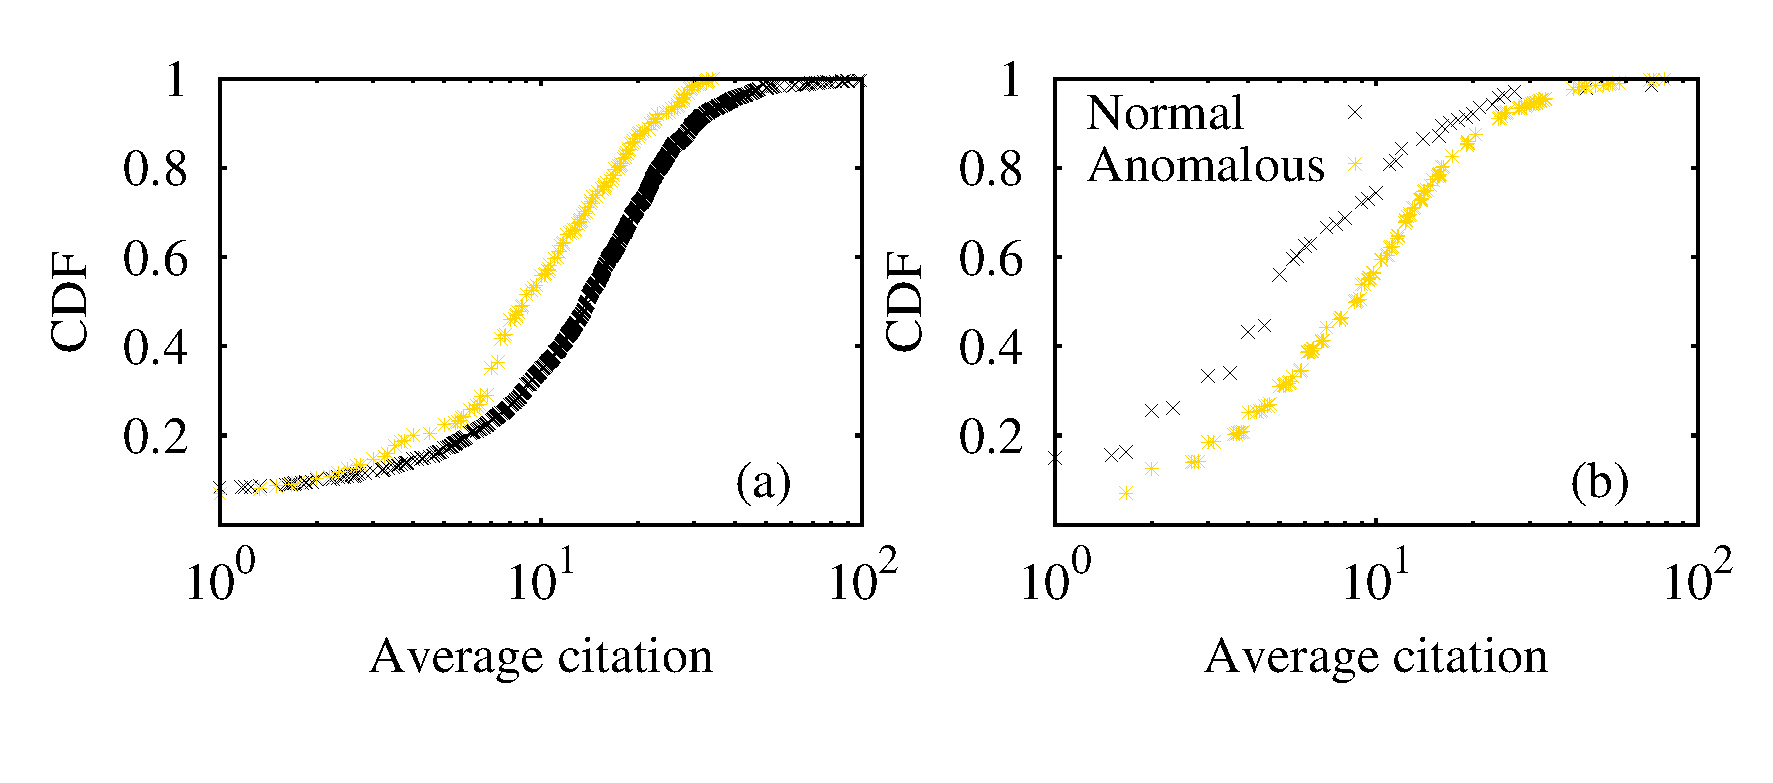
\includegraphics[scale=0.27]{./texfiles/Chapter_4/cikm/figures/reviewer_all_anom.eps}
\caption{\label{rev_pred}Cumulative distribution function of the average citations for the two sets of reviewers (anomalous and normal).\vspace{4mm}}
\vspace{3mm}
\end{figure}
%Thus, using the above features we were able to identify the anomalous reviewers and editors. We believe our method could be useful in further improving the peer-review process. Moreover it could be useful in assisting editors to select reviewers as well as administrators in selecting editors. 
\medskip